\section{Spezielle Verteilungen}
\label{sec:spezielle_verteilungen}
\subsection{Diskrete und stetige Verteilungen}
\label{subsec:diskrete_stetige_verteilungen}
\begin{center}
    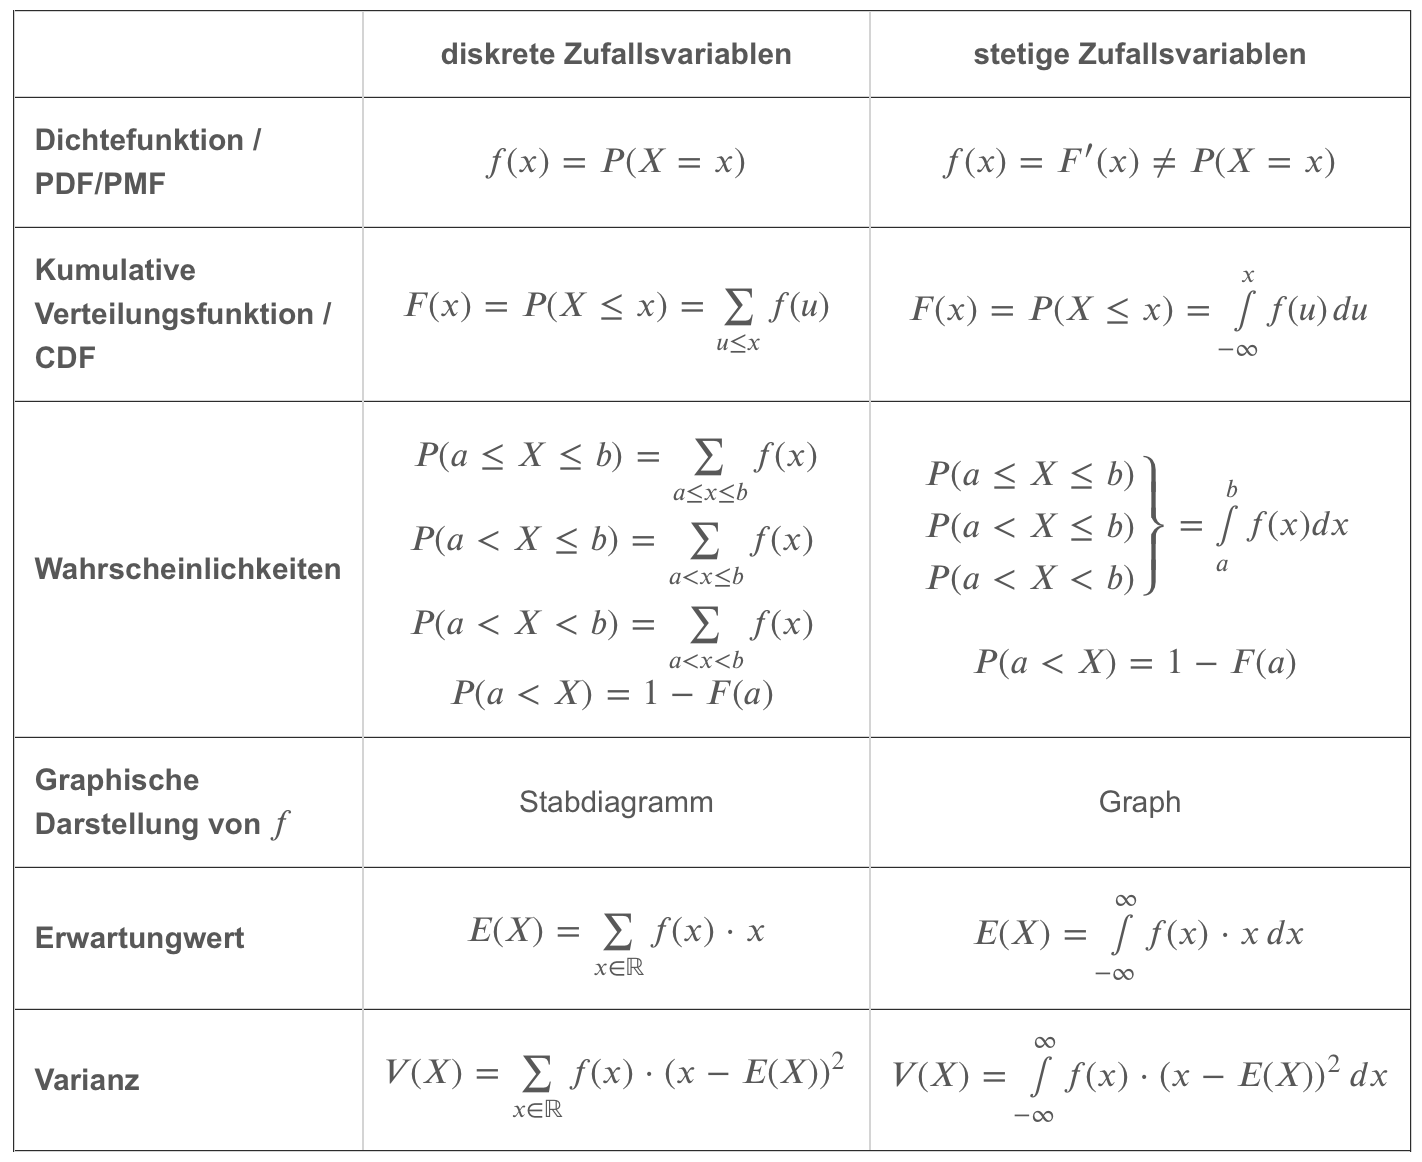
\includegraphics[width=1\linewidth]{images/tabelle1.png}
\end{center}
\begin{center}
    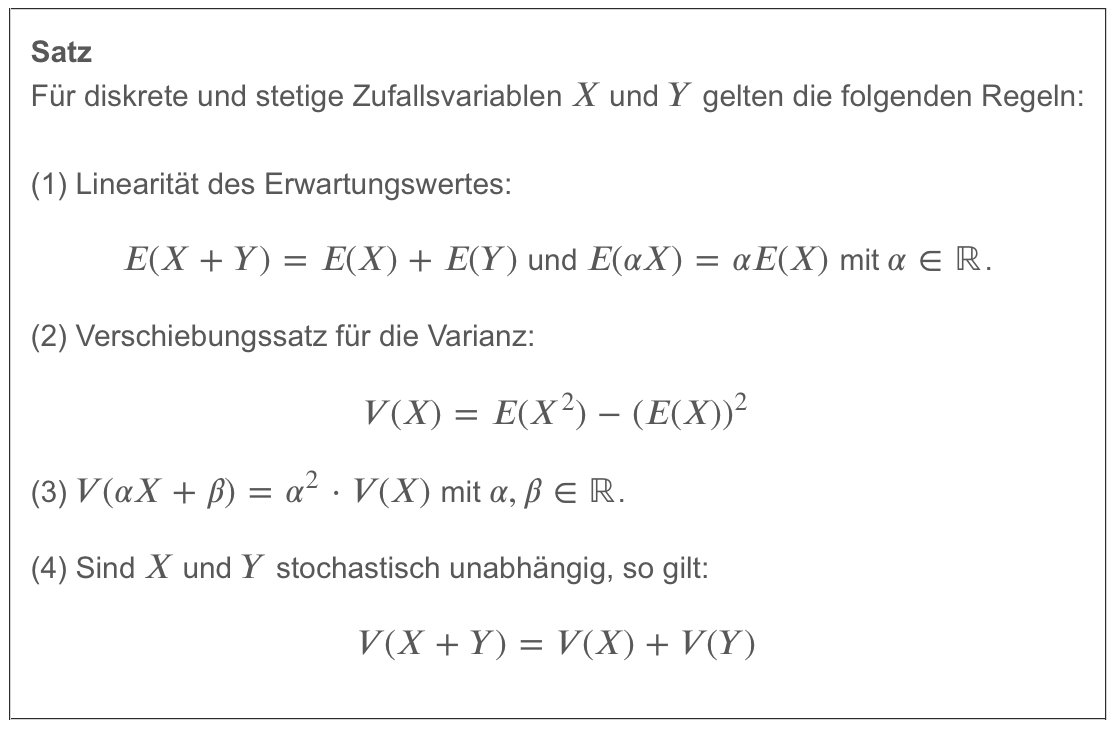
\includegraphics[width=0.8\linewidth]{images/satz.png}
\end{center}
Es ist effizienter, die Varianz mithilfe des Verschiebungssatzes zu berechnen als mithilfe der Definition.
\subsection{Die Hypergeometrische Verteilung}
\label{subsec:hypergeometrische_verteilung}
Eine diskrete Zufallsvariable $X$ heisst \textit{hypergeometrisch verteilt} mit den Parametern $n$ (Anzahl Ziehungen ohne Zurücklegen),
$N$ (Gesamtzahl aller Objekte) und $M$ (Gesamtzahl aller Merkmalsträger), wenn ihre Dichtefunktion (PMF) gegeben ist durch:
\begin{equation*}
    P(X = x) = \frac{\binom{M}{x}\binom{N-M}{n-x}}{\binom{N}{n}}
\end{equation*}
Schreibweise: $X \sim H(N, M, n)$ \\
$X$ zählt, wie oft bei der $n$-fachen Ziehung (nacheinander und ohne Zurücklegen) ein Merkmalsträger gezogen wird.
\begin{center}
    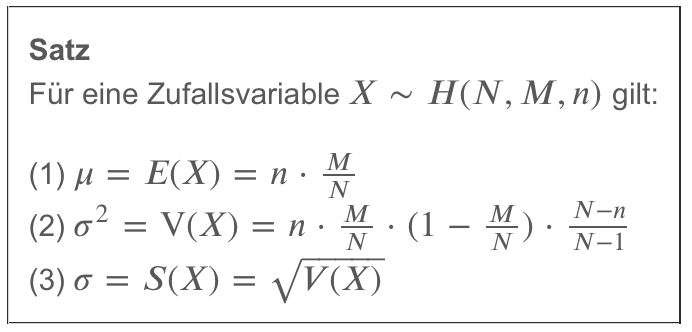
\includegraphics[width=0.5\linewidth]{images/satz2.png}
\end{center}
\subsection{Die Bernoulli-Verteilung}
\label{subsec:bernoulli_verteilung}
Eine Zufallsvariable $X$ heisst \textit{Bernoulli-verteilt}, wenn sie nur zwei verschiedene Werte annehmen kann: den Wert 1 mit der Wahrscheinlichkeit
$P(X = 1) = p$ und den Wert 0 mit der Wahrscheinlichkeit $P(X = 0) = 1 - p$. \\
\begin{center}
    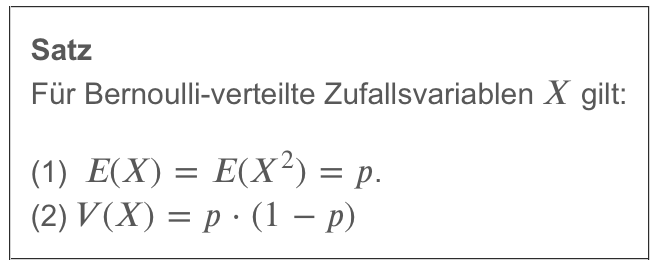
\includegraphics[width=0.5\linewidth]{images/satz3.png}
\end{center}
\subsection{Die Binominalverteilung}
\label{subsec:binominalverteilung}
Eine diskrete Zufallsvariable $X$ heisst binomialverteilt mit den Parametern $n$ (Anzahl Wiederholungen) und $p$ (Wahrscheinlichkeit für ein Ergebnis 1), 
wenn ihre Dichtefunktion (PMF) gegeben ist durch:
\begin{equation*}
    P(X = x) = \binom{n}{x}p^x(1-p)^{n-x}
\end{equation*}
Schreibweise: $X \sim B(n; p)$ \\
$X$ zählt, wie oft bei $n$ Wiederholungen eines Bernoulli-Experiments das Ergebnis 1 eintritt. Die Wahrscheinlichkeit für das Ergebnis 0 wird
üblicherweise mit $q = 1 - p$ bezeichnet. \\
Die $B(n; p)$-verteilte Zufallsvariable $X$ kann als Summe von $n$ Bernoulli-verteilten Zufallsvariablen $X_i$ aufgefasst werden: $X=\sum_{i=1}^n X_i$.
Dabei hält $X_i$ das Ergebnis des $i$-ten Experiments fest, und es gilt: $P(X_i = 1) = p$.
\begin{center}
    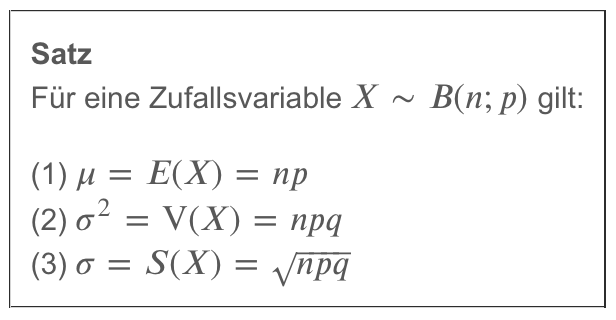
\includegraphics[width=0.5\linewidth]{images/satz4.png}
\end{center}
\subsubsection{Faustregel zur Approximation}
\label{subsubsec:faustregel_approximation}
Wenn die Bedingung $n \leq \frac{N}{20}$ erfüllt ist, kann die Hypergeometrische Verteilung $H(N, M, n)$ durch die Binomialverteilung $B(n, \frac{M}{N})$
approximiert werden. \\
\begin{equation*}
    H(N,M,n) \approx B(n, \frac{M}{N})
\end{equation*}
\subsection{Die Poisson-Verteilung}
\label{subsec:poisson_verteilung}
Eine diskrete Zufallsvariable $X$ heisst \textit{poissonverteilt} mit dem Parameter $\lambda > 0$ (durchschnittliche Anzahl Ereignisse pro betrachtetes Zeitintervall),
wenn ihre Dichtefunktion (PMF) gegeben ist durch:
\begin{equation*}
    P(X = x) = \exp(-\lambda)\frac{\lambda^x}{x!}
\end{equation*}
Schreibweise: $X \sim Poi(\lambda)$ \\
$X$ zählt die Anzahl der (stochastisch unabhängigen, gleichartigen) Ereignisse in einem betrachteten Zeitintervall. \\
\begin{center}
    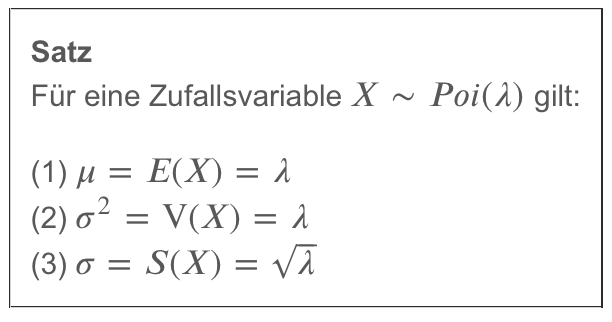
\includegraphics[width=0.5\linewidth]{images/satz5.png}
\end{center}
\subsubsection{Faustregel zur Approximation}
\label{subsubsec:faustregel_approximation}
Wenn die Bedingung $n \leq 50$ und $p \leq 0.1$ erfüllt ist, kann die Binominalverteilung $B(n,p)$ gut durch die Poissonverteilung
$Poi(np)$ approximiert werden:
\begin{equation*}
    B(n,p) \approx Poi(np)
\end{equation*}
\subsection{Die Gauss'sche Normalverteilung}
\label{subsec:gauss_sche_normalverteilung}
Eine stetige Zufallsvariable $X$ heisst \textit{normalverteilt} mit den Parametern $\mu$ (Erwartungswert) und $\sigma^2$ (Varianz) ($\sigma > 0$),
wenn sie folgende Dichtefunktion (PDF) hat:
\begin{equation*}
    \phi_{\mu, \sigma}(x) = \frac{1}{\sqrt{2\pi\sigma}}\exp(-\frac{1}{2}(\frac{x-\mu}{\sigma})^2)
\end{equation*}
Schreibweise: $X \sim N(\mu;\sigma)$ \\
\begin{center}
    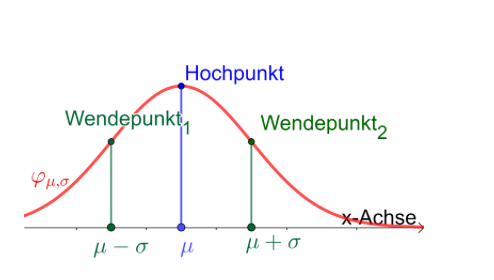
\includegraphics[width=0.5\linewidth]{images/gauss.png}
\end{center}
Die kumulative Verteilungsfunktion (CDF) von $\phi_{\mu, \sigma}(x)$ wird mit $\Phi_{\mu, \sigma}(x)$ bezeichnet und ist gegeben durch:
\begin{equation*}
    \Phi_{\mu, \sigma}(x) = \int_{-\infty}^x \phi_{\mu, \sigma}(t)dt = \frac{1}{\sqrt{2\pi}\sigma}\cdot\int_{-\infty}^x 
    \exp(-\frac{1}{2}(\frac{t-\mu}{\sigma})^2)dt
\end{equation*}
\begin{center}
    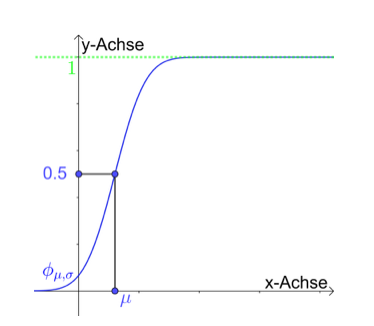
\includegraphics[width=0.5\linewidth]{images/gauss2.png}
\end{center}
Ist $\mu = 0$ und $\sigma = 1$, so spricht man von der Standardnormalverteilung. Ihre Dichtefunktion (PDF) wird mit $\phi$ bezeichnet; sie ist gegeben durch:
\begin{equation*}
    \phi(x) = \frac{1}{\sqrt{2\pi}}\exp(-\frac{1}{2}x^2)
\end{equation*}
Ihre Verteilungsfunktion (CDF) $\Phi(x)_{0,1}(x)$ wird mit $\Phi(x)$ bezeichnet. \\
Schreibweise: $X \sim N(0;1)$ \\
Die Verteilungsfunktion der Normalverteilung kann nicht auf elementare Weise berechnet werden. 
Für ihre Werte gibt es Tabellen (Papula 12. Aufl. S. 514); die Tabellen beziehen sich allerdings immer auf die Standardnormalverteilung.
\subsubsection{Bemerkungen zur Dichtefunktion der Normalverteilung}
\label{subsubsec:bemerkungen_dichtefunktion_normalverteilung}
Die Dichtefunktion (PDF) $\phi_{\mu, \sigma}(x)$ hat folgende Eigenschaften:
\begin{itemize}
    \item Sie ist symmetrisch bezüglich der Geraden $y = \mu$
    \item Sie hat Wendepunkte an den Stellen $\mu - \sigma$ und $\mu + \sigma$
    \item Sie ist normiert, d.h. es gilt:
    \begin{equation*}
        \int_{-\infty}^{\infty}\phi_{\mu, \sigma}(x)dx = \frac{1}{\sqrt{2\pi}\sigma} \cdot \int_{-\infty}^{\infty}\exp(-\frac{1}{2}(\frac{x-\mu}{\sigma})^2)dx = 1
    \end{equation*}
    \item Eine Änderung von $\mu$ bewirkt eine Verschiebung in $x$-Richtung; je grösser $\sigma$ ist, desto breiter und niedriger wird die Glockenkurve
    \item Für eine Zufallsvariable $X \sim N(\mu;\sigma)$ gilt: $E(X) = \mu$ und $V(X) = \sigma^2$
\end{itemize}
Bei einer Zufallsvariable $X$, die der Normalverteilung $N(\mu;\sigma)$ folgt, liegen:
\begin{itemize}
    \item ca. $68\%$ der Werte zwischen $\mu - \sigma$ und $\mu + \sigma$
    \item ca. $95\%$ der Werte zwischen $\mu - 2\sigma$ und $\mu + 2\sigma$
    \item ca. $99.7\%$ der Werte zwischen $\mu - 3\sigma$ und $\mu + 3\sigma$
\end{itemize}
\begin{center}
    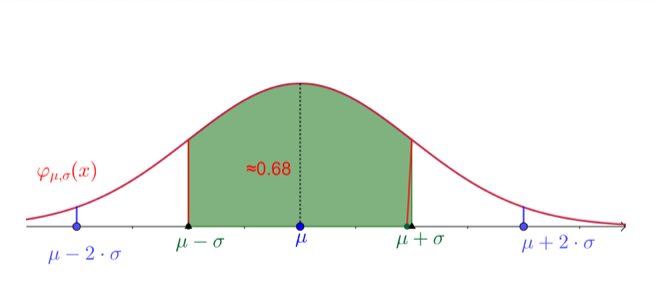
\includegraphics[width=0.5\linewidth]{images/normalverteilung.png}
\end{center}
\begin{center}
    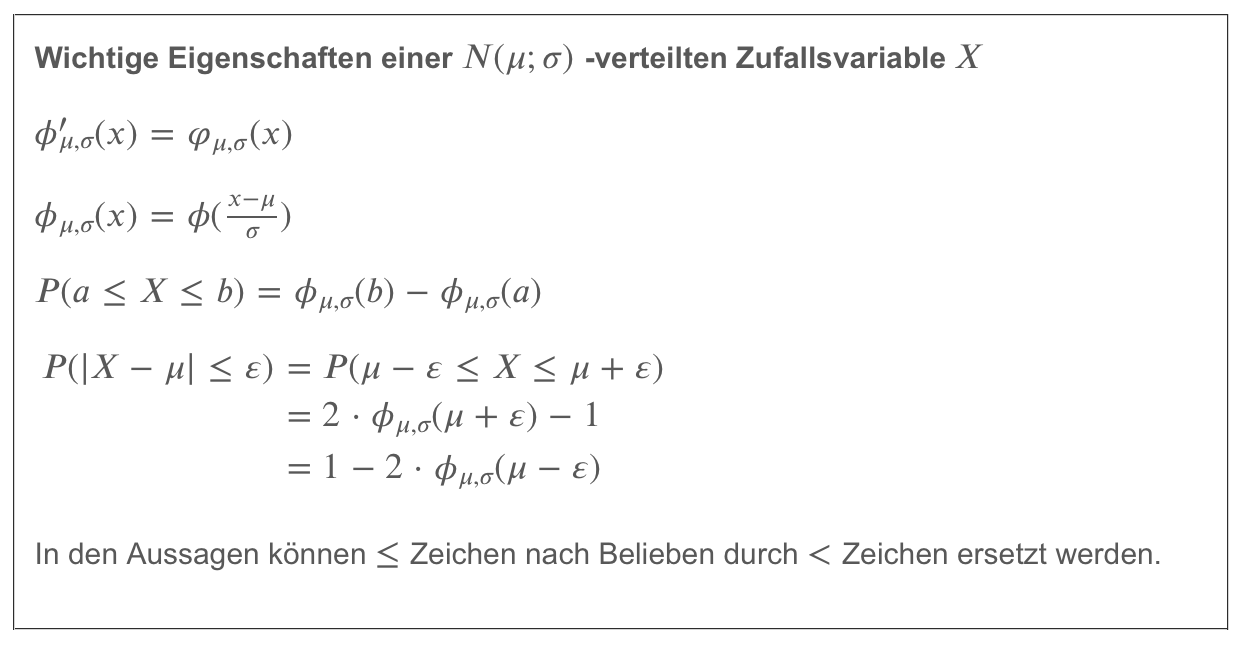
\includegraphics[width=0.8\linewidth]{images/normalverteilung2.png}
\end{center}
\begin{center}
    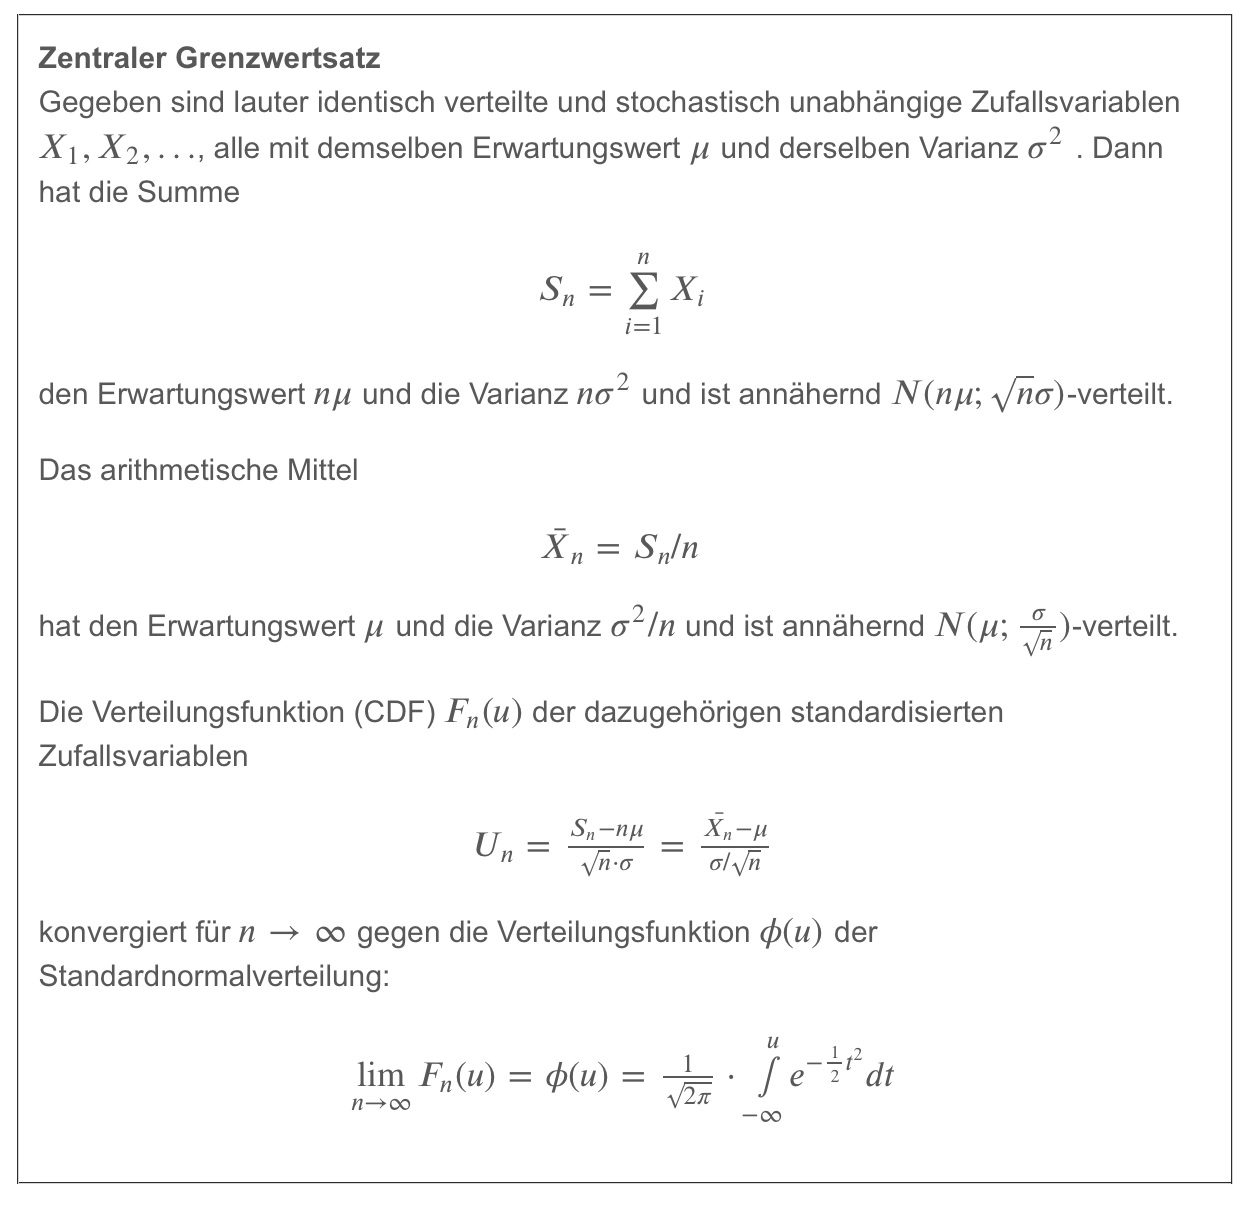
\includegraphics[width=1\linewidth]{images/normalverteilung3.png}
\end{center}